\section{Method} \label{sec:method}
In this section we will go through the algorithm used to determine the musical key.
As stated before, we will make use the MKC proposed by \citeauthor{krumhansl2001cognitive} in \cite{krumhansl2001cognitive}.


The Krumhansl-Schmuckler algorithm is based on key profiles.
Each one of the 24 possible keys (A-G\#, Major and Minor) will have its own profile.
Each profile is a vector of 12 values, each of them corresponding to a note in the chromatic scale. (A-G\#).
The profile was created based on data from experiments by Krumhansl and Kessler \cite{krumhansl1982tracing}.
In these experiments, participants where asked to rate how well a note fitted a musical element like a scale, chord and cadence, associated with a key.
We these ratings, a weighted value was given to each note. The experiment was repeated for all keys.

\begin{figure}[H]
    \centering
    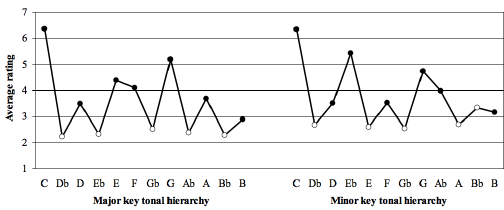
\includegraphics[width=.8\linewidth]{figs/method/key_profiles_C.png}
    \caption{Key profiles for C Major and C Minor by Krumhansl \& Kessler’s (1982)}
    \label{fig:key_profiles_c}
\end{figure}

As we can observe in figure \ref{fig:key_profiles_c}, in both profiles, the \textbf{tonic} note (C) is given the highest weight.
This is because it is the most important note, with music being composed around it. It is therefore, the outcome that our ear is expecting naturally for example, in a cadence.

Another highly important note is the \textbf{dominant} note, in this case G for both of them.
The dominant is the note that effectively enables us to identify the key of the piece(A-G\#).
It it part of the tonic chord, and when we hear the dominant note/chord, we expected it to lead to the tonic note/chord, which we call the perfect cadence.

Finally, we can also pinpoint the \textbf{mediant} note. The mediant is the note that differentiates a major and minor key in the same note.
In the case, the mediant is E and Eb for C Major and C Minor respectively. This note is also part of the tonic chord, and theoretically, it can render the dominant note useless as it also identifies the key.
Switching the dominant for the mediant is, in fact, a very common composition technique in Jazz.
It tends to have a more significant role in a a minor key as, with only the tonic and dominant notes, we tend to assume the key is major.
Therefore, its recursive use is necessary to define the key as minor.

Went the data was collected for all keys, it was noticed that there was little variation between major keys (after adjusting for transposition).
For example, in C major, C weighted 6.35 and C\# 2.23, whereas in C\# major, C\# weighted 6.35 and D 2.23.
For this matter, the values were averaged over all major keys, creating a profile that was used in all major keys.
The same was done for minor keys.

In order to compare the piece with the different profiles, we to create a vector of 12 inputs. Each input corresponds to the total duration of the pitch (A-G\#) in the piece.
Of course, the values obtained depend on the tempo at which the piece is being played at.
However, every value will scale proportionately with the tempo, therefore affecting the output value but not the output prediction.

The correlation between the input vector and each profile is given by:


\begin{center}
    \centering
    \(r = \frac{\sum{(x-\overline{x})(y-\overline{y})}}{(\sum{(x-\overline{x})^2(y-\overline{y})^2})^{1/2}}\)
\end{center}

where \(x = \) is the input vector values, \(\overline{x} = \) the average input vector values,
\(y = \) the key-profile values for a given key and \(\overline{y} = \) the average key-profile values for that key.

The calculation must be done for all key profiles, and the one that yields the highest value is the preferred key.

In \cite{Temperley2004Musicp}, \citeauthor{Temperley2004Musicp} calculated the input vector values for a small melody called "Yankee Doodle":

\begin{figure}[H]
    \centering
    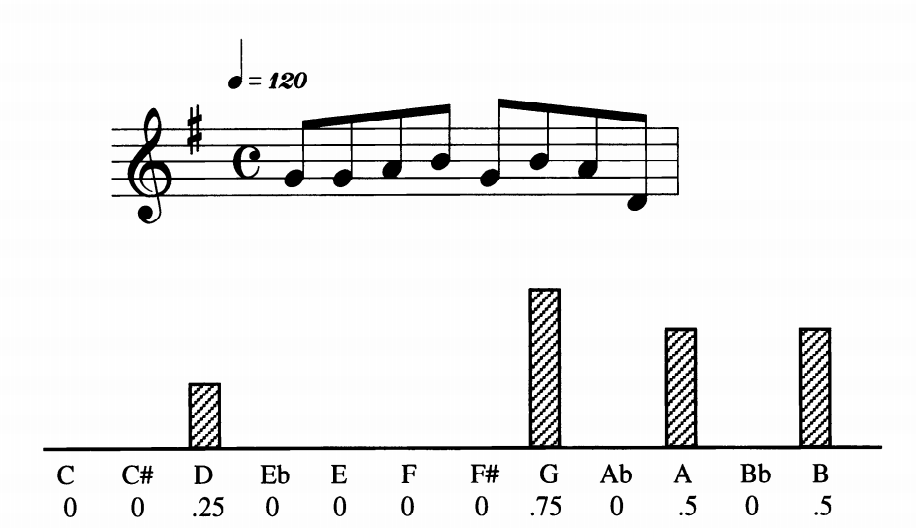
\includegraphics[width=.8\linewidth]{figs/method/yankee_song.png}
    \caption{Measure of "Yankee Doodle," with input vector showing total duration of each pitch class}
    \label{fig:yankee_song}
\end{figure}

The correlation values obtained for each key profile are the following:

\begin{table}[H]
    \centering
    \begin{tabular}{c c}
        \multicolumn{2}{c}{\large{Key Profile Scores}}\\
        \hline
        Key & Score\\
        \hline
        C major & 0.245\\
        C minor & -0.012\\
        C\# major & -0.497\\
        C\# minor & -0.296\\
        D major & 0.485\\
        D minor & 0.133\\
        D\# major & -0.114\\
        D\# minor & -0.354\\
        E major & 0.000\\
        E minor & 0.398\\
        F major & 0.003\\
        F minor & -0.384\\
        F\# major & -0.339\\
        F\# minor & 0.010\\
        \textbf{G major} & \textbf{0.693}\\
        G minor & 0.394\\
        G\# major & -0.432\\
        G\# minor & -0.094\\
        A major & 0.159\\
        A minor & 0.223\\
        A\# major & -0.129\\
        A\# minor & -0.457\\
        B major & -0.061\\
        B minor & -0.436\\
        \hline \\[0.1ex]
    \end{tabular}
    \caption{}
    \label{table:1}
\end{table}

As it is observed in table \ref{table:1}, \textbf{G major} is the preferred key. 
In fact, it is the correct answer.
This is a relative simple example, as all the notes in the excerpt are in the G major scale.
Also, the tonic and mediant notes have a significant presence, and its dominant is also present, making it very obvious for the algorithm.
